\documentclass[11pt]{article}
\usepackage{graphicx} %for displaying images
\usepackage{float}
\usepackage{listings}
\usepackage{color}


\definecolor{dkgreen}{rgb}{0,0.6,0}
\definecolor{gray}{rgb}{0.5,0.5,0.5}
\definecolor{mauve}{rgb}{0.58,0,0.82}

\lstset{frame=tb,
	language=Python,
	aboveskip=3mm,
	belowskip=3mm,
	showstringspaces=false,
	columns=flexible,
	basicstyle={\small\ttfamily},
	numbers=none,
	numberstyle=\tiny\color{gray},
	keywordstyle=\color{blue},
	commentstyle=\color{dkgreen},
	stringstyle=\color{mauve},
	breaklines=true,
	breakatwhitespace=true,
	tabsize=3
}

%----------------------------------------------------------------------------------------
%	TITLE SECTION
%----------------------------------------------------------------------------------------
\title{	
	\normalfont\normalsize
	\textsc{Old Dominion University}\\ % Your university, school and/or department name(s)
	\vspace{25pt} % Whitespace
	\rule{\linewidth}{0.5pt}\\ % Thin top horizontal rule
	\vspace{20pt} % Whitespace
	{\huge Assignment Five}\\ % The assignment title
	\vspace{12pt} % Whitespace
	\rule{\linewidth}{2pt}\\ % Thick bottom horizontal rule
	\vspace{20pt} % Whitespace
}
\author{\LARGE Joshua Gahan} % Your name
\date{\normalsize\today} % Today's date (\today) or a custom date

\begin{document}
	\pagenumbering{gobble}
	\maketitle %render title
	\newpage
	\pagenumbering{arabic}
	
	\section{Karate Club, comparision of algorithm performance with historical data. }
	\hspace{10mm} We populated a graph with data from the Zachary's Karate Club study and then we applied Girvan-Newman's algorithm to split the group into two distinct communities. We then compared the results of our graph post split to the real data provided in the study to compare the accuracy of algorithm in predicting how communities might split up, given the relations between the members of the community. \\
	\hspace{10mm} We began by reading the known data in and populating our nodes. We chose to color the nodes based on the way that the community split up in the real study. Members of Mr Hi's community have had their nodes colored red, and members of John's community have had their nodes colored green. Mr. Hi and John's nodes where named HI and JA respectively.  \\
	\hspace{10mm} We utilized the networkx library to manage our nodes and edges, and used matplotlib to draw our graphs. 
	\subsection{Implementation of Girvan\_Newman Algorithm. }
	\begin{lstlisting}
	for url in data:
	    savefile_counter = 0
	    
	    
	    all_members = set(range(34))
	    club1 = {0, 1, 2, 3, 4, 5, 6, 7, 8, 10, 11, 12, 13, 16, 17, 19, 21}
	    
	    G = nx.Graph()
	    G.add_nodes_from(all_members)
	    G.name = "Zachary's Karate Club"
	    
	    # data read in here
	    #
	    #
	    
	    color_map = []
	    for node in G:
	        if node in club1:
	            color_map.append('green')
	        else:
	            color_map.append('red')
	    
	    labeldict = {}
	    edgedict = []
	    for i in range (0,len(G)):
	        labeldict[i] = i
	    
	    for i in range (0,len(G.edges)):
	        edgedict.append('black')
	    
	    print(G.edges)
	    
	    labeldict[0] = "JA"
	    labeldict[33] = "HI"
	    
	    
	    nx.draw(G, node_color = color_map, edge_color=edgedict, width=2, labels=labeldict, with_labels=True)
	    plt.show()
	    plt.savefig('./graph/karate%s.png' % savefile_counter)
	    
	    
	    graphs = list(nx.connected_component_subgraphs(G))	    
	    while len(graphs) == 1:
	        betweeness = nx.edge_betweenness(G, 34, normalized=True)
	        sort = sorted(betweeness.items(), key=lambda x: x[1])
	    
	        leading_edge = sort[len(sort) - 1][0]
	    
	        edge_counter = 0
	        for u, v in G.edges:
	            if (u == leading_edge[0] and v == leading_edge[1]):
	                edgedict[edge_counter] = 'blue'
	                nx.draw(G, node_color=color_map, edge_color=edgedict, width=2, labels=labeldict, with_labels=True)
	                plt.show()
	                del edgedict[edge_counter]
	                G.remove_edge(u, v)
	                nx.draw(G, node_color=color_map, edge_color=edgedict, width=2, labels=labeldict, with_labels=True)
	                plt.show()
	                break
	           else:
	               pass
	           edge_counter += 1
	    graphs = list(nx.connected_component_subgraphs(G))
	\end{lstlisting}
	\hspace{10mm} We start off by creating 34 nodes which will later be populated with data. the numbers in club1 represent real-life individuals who stayed with John upon the clubs split. The nodes are id'd between 0 and 33, representing the 34 members of the original club. Thus, node 3 would be not only the third node, but would have '3' as its unique identifier. \\ 
	\hspace{10mm}We then create a color\_map list to which we append either "red" or "green" depending on if the the respective node id is equal to one of the numbers in club1. This color list will be used during plotting to color our nodes appropriately. We performed similar operation to populate labeldict and edgedict which are the node labels and the edge colors respectively. Utilizing these helper lists, we then draw our graph. \\
	\hspace{10mm} We then come to the heart of the algorithm. Nx.connected.. returns an array containing each component in the graph, we take advantage of this by making the length of the connected array the condition of our while loop.  \\
	\hspace{10mm} Within the loop, we utilize nx.edge\_betweeness to calculate the betweeness of each of our edges. Once calculated, we sort the returned betweeness dictionary such that the item with the highest betweeness is the last item in the list. This dictionary has a tuple of nodes as its keys, and here we search for the edge that has both of the leading\_edge tuple as its parents. We then color this edge blue for display and then remove the edge.  \\
	\hspace{10mm} We create two additional plots. for each iteration through the while loop, representing the graph with the edge to be deleted colored blue, and then the edge removed in the next plot. \\
	
	\section{Findings}
	\hspace{10mm}  We have found that the Girvan-Newman algorithm does indeed do a very good job of predicting the split in the social graph. In the original study, Zachary managed to correctly predict how all but one of the members would split when the karate club broke up. The Girvan-Newman algorithm in our implementation successfully predicted how all but two members (two and eight) would break. Given the sheer number of variables that could affect a split in real life such as what this study followed, the algorithm performs amazingly well given that it simply operates by breaking edges depending on the degree of betweeness between nodes. 
	\section{D3}
	\hspace{10mm} A implementation showing the splitting of this graph along historical lines has been provided as one file labeled index.html. This implementation does not utilize the algorithm, but rather simply breaks according to the data provided. You will operate it by clicking the provided button multiple times, each time removing a single relevant edge. 
	
	\section{The algorithm at work}
	What follows is a series of images, that shows the algorithm at work. Below a full showing of the algorithm splitting the karate club into 2 groups is example images which show the group ran through the same algorithm after being split into 3,4,5,6, and 10 nodes. 
	\begin{figure}[h!]
		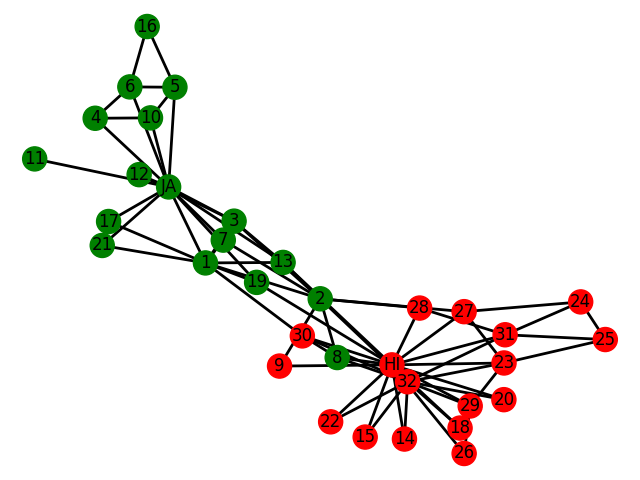
\includegraphics[scale=0.5]{resources/myplot17.png}
		\caption{Graphical visualization of the algorithm at work }
	\end{figure}
	\begin{figure}[h!]
		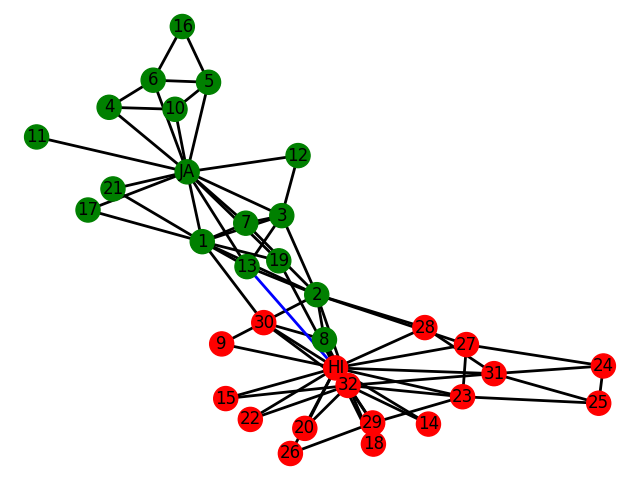
\includegraphics[scale=0.5]{resources/myplot16.png}
		\caption{Graphical visualization of the algorithm at work }
	\end{figure}
	\begin{figure}[h!]
		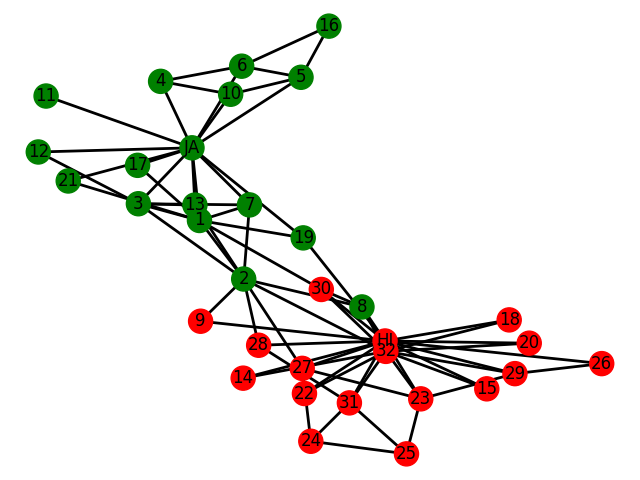
\includegraphics[scale=0.5]{resources/myplot15.png}
		\caption{Graphical visualization of the algorithm at work }
	\end{figure}
	\begin{figure}[h!]
		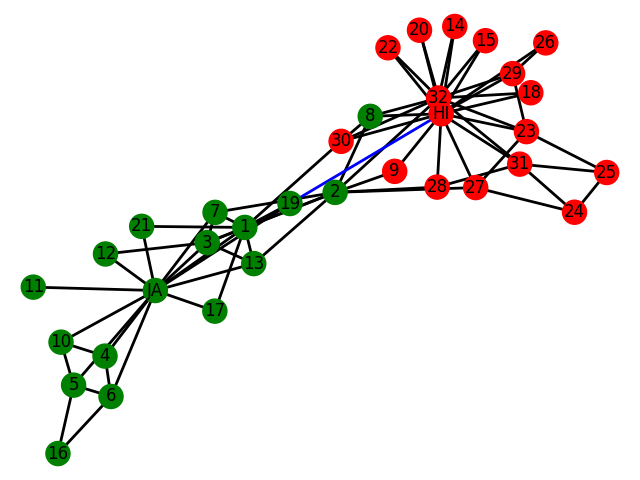
\includegraphics[scale=0.5]{resources/myplot14.png}
		\caption{Graphical visualization of the algorithm at work }
	\end{figure}
	\begin{figure}[h!]
		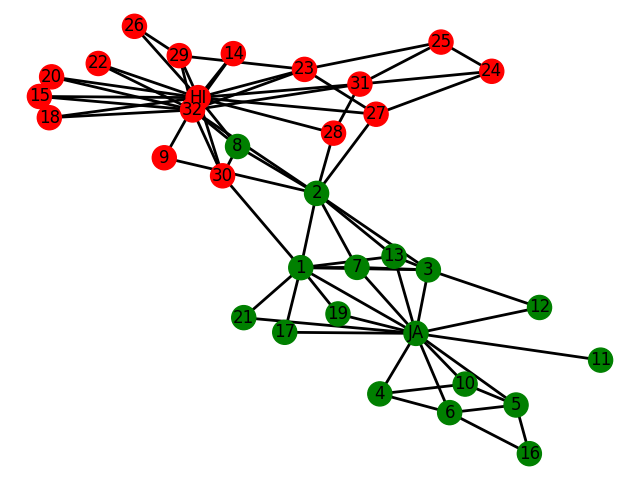
\includegraphics[scale=0.5]{resources/myplot13.png}
		\caption{Graphical visualization of the algorithm at work }
	\end{figure}
	\begin{figure}[h!]
		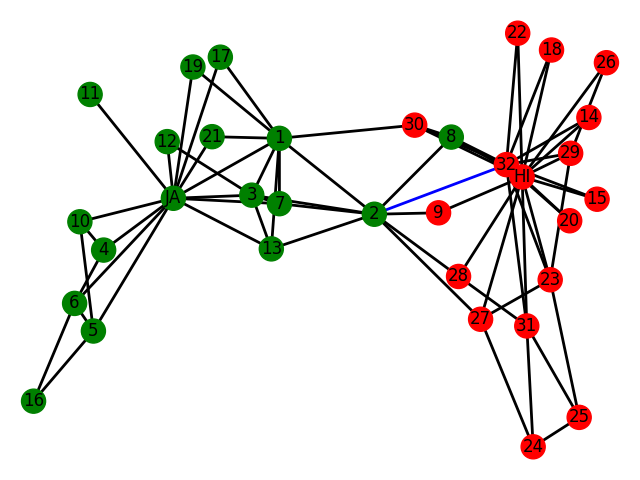
\includegraphics[scale=0.5]{resources/myplot12.png}
		\caption{Graphical visualization of the algorithm at work }
	\end{figure}
	\begin{figure}[h!]
		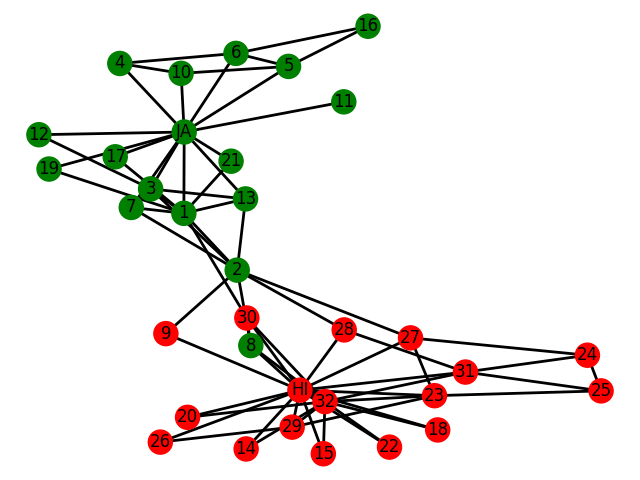
\includegraphics[scale=0.5]{resources/myplot11.png}
		\caption{Graphical visualization of the algorithm at work }
	\end{figure}
	\begin{figure}[h!]
		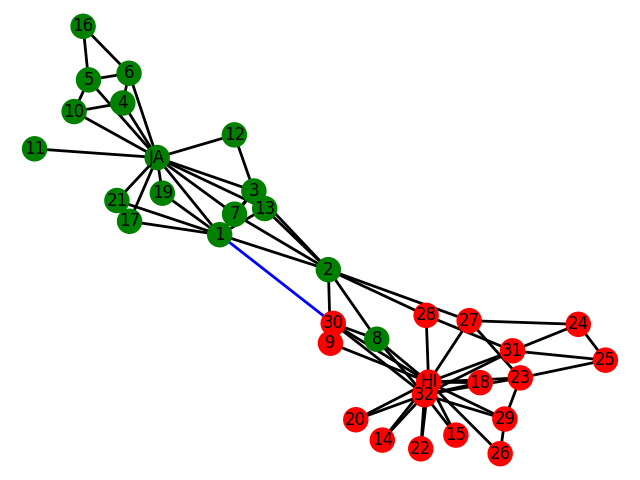
\includegraphics[scale=0.5]{resources/myplot10.png}
		\caption{Graphical visualization of the algorithm at work }
	\end{figure}
	\begin{figure}[h!]
		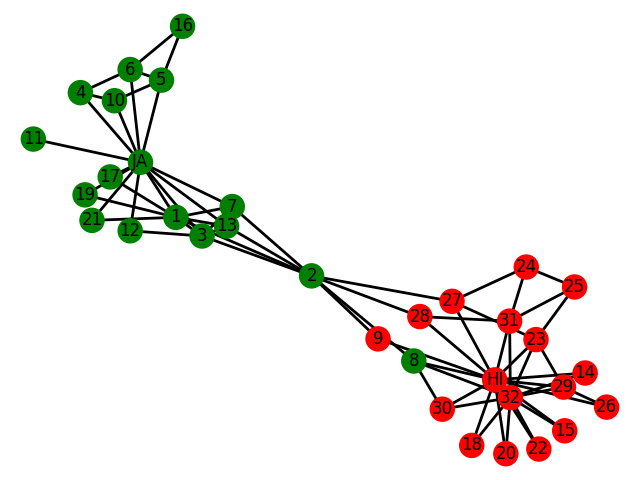
\includegraphics[scale=0.5]{resources/myplot9.png}
		\caption{Graphical visualization of the algorithm at work }
	\end{figure}
	\begin{figure}[h!]
		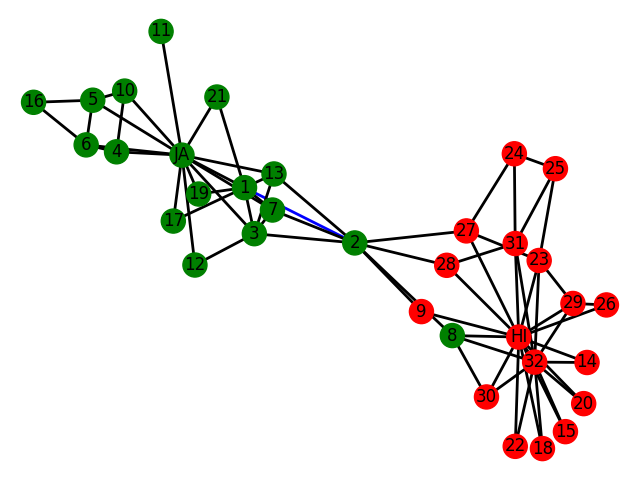
\includegraphics[scale=0.5]{resources/myplot8.png}
		\caption{Graphical visualization of the algorithm at work }
	\end{figure}
	\begin{figure}[h!]
		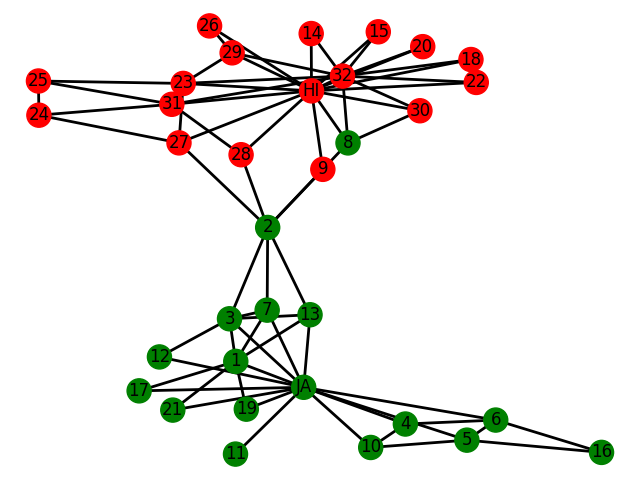
\includegraphics[scale=0.5]{resources/myplot7.png}
		\caption{Graphical visualization of the algorithm at work }
	\end{figure}
	\begin{figure}[h!]
		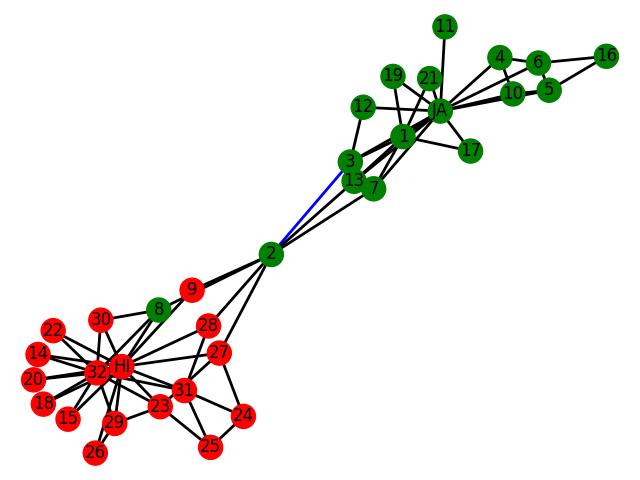
\includegraphics[scale=0.5]{resources/myplot6.png}
		\caption{Graphical visualization of the algorithm at work }
	\end{figure}
	\begin{figure}[h!]
		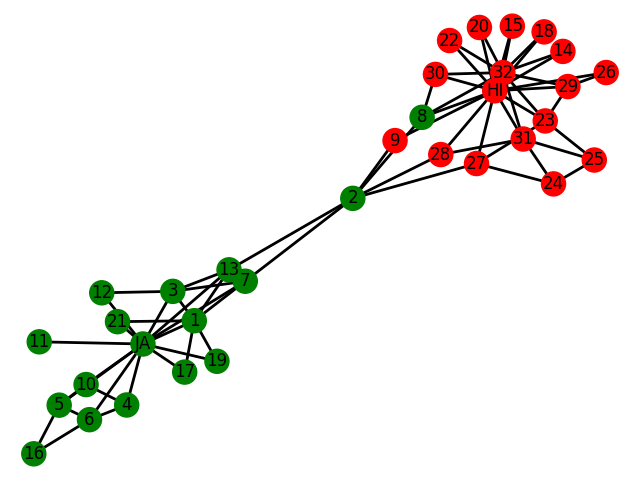
\includegraphics[scale=0.5]{resources/myplot5.png}
		\caption{Graphical visualization of the algorithm at work }
	\end{figure}
	\begin{figure}[h!]
		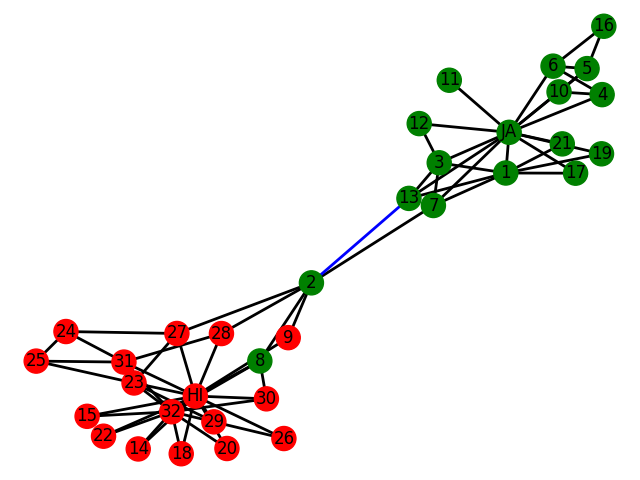
\includegraphics[scale=0.5]{resources/myplot4.png}
		\caption{Graphical visualization of the algorithm at work }
	\end{figure}
	\begin{figure}[h!]
		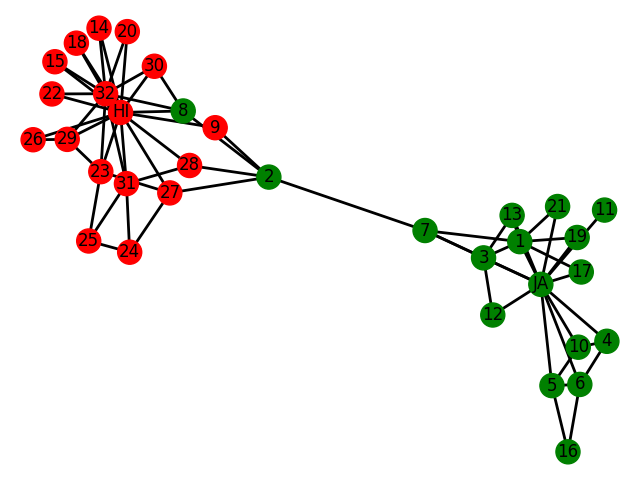
\includegraphics[scale=0.5]{resources/myplot3.png}
		\caption{Graphical visualization of the algorithm at work }
	\end{figure}	
	\begin{figure}[h!]
		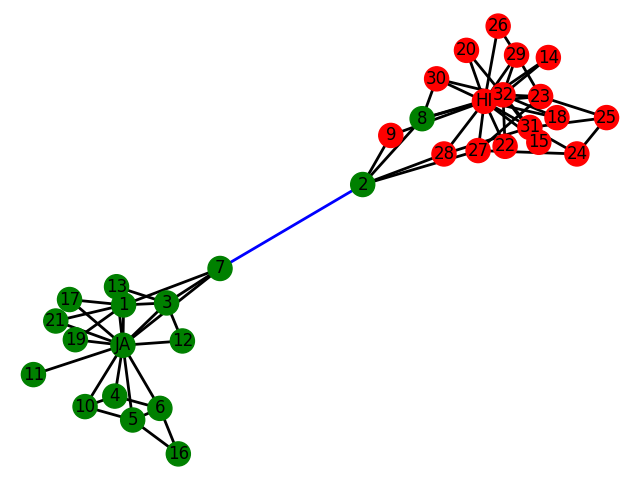
\includegraphics[scale=0.5]{resources/myplot2.png}
		\caption{Graphical visualization of the algorithm at work }
	\end{figure}
	\begin{figure}[h!]
		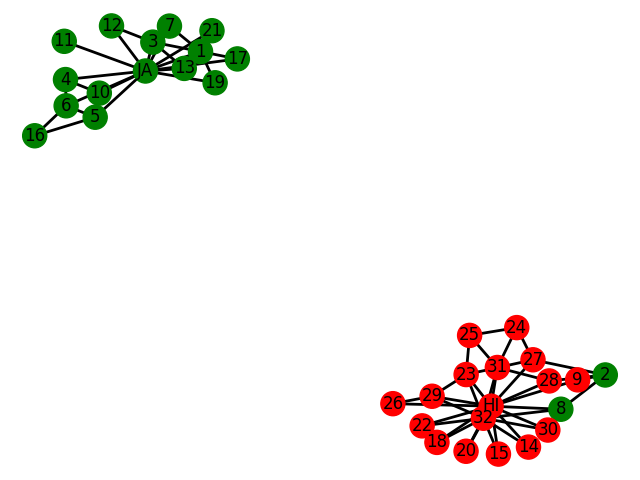
\includegraphics[scale=0.5]{resources/myplot1.png}
		\caption{Graphical visualization of the algorithm at work }
	\end{figure}
	\begin{figure}[h!]
		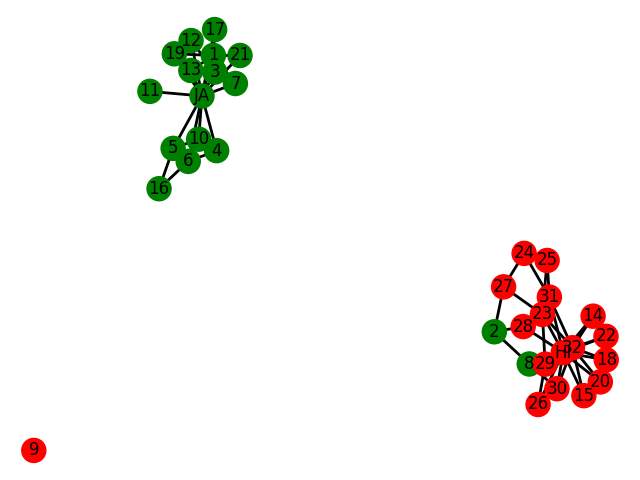
\includegraphics[scale=0.5]{resources/myplot18.png}
		\caption{Split into 3 nodes }
	\end{figure}
	\begin{figure}[h!]
		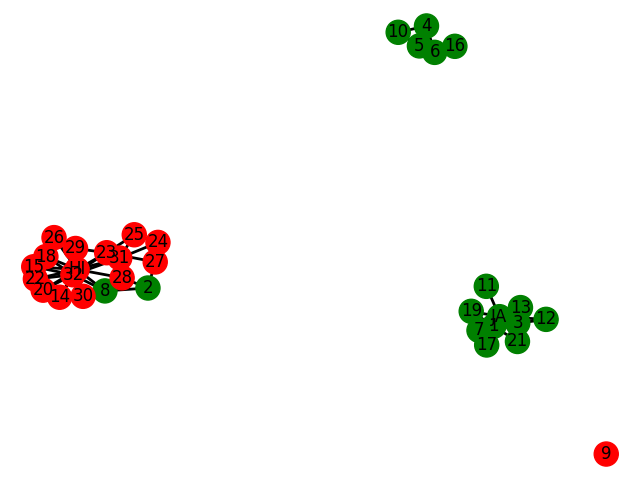
\includegraphics[scale=0.5]{resources/myplot19.png}
		\caption{split into 4 nodes }
	\end{figure}	
	\begin{figure}[h!]
		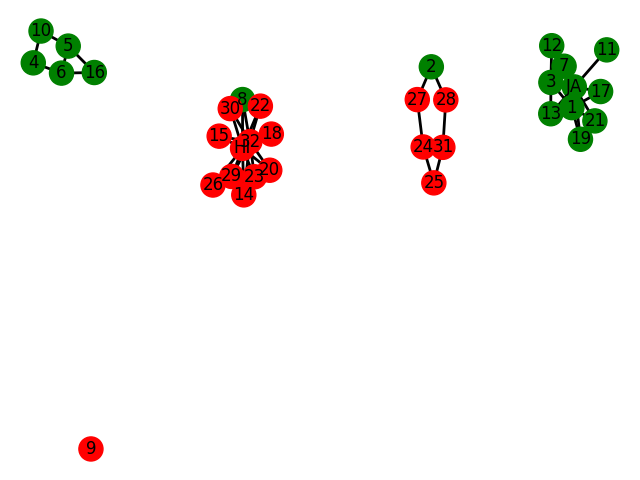
\includegraphics[scale=0.5]{resources/myplot20.png}
		\caption{Split into 5 nodes }
	\end{figure}
	\begin{figure}[h!]
		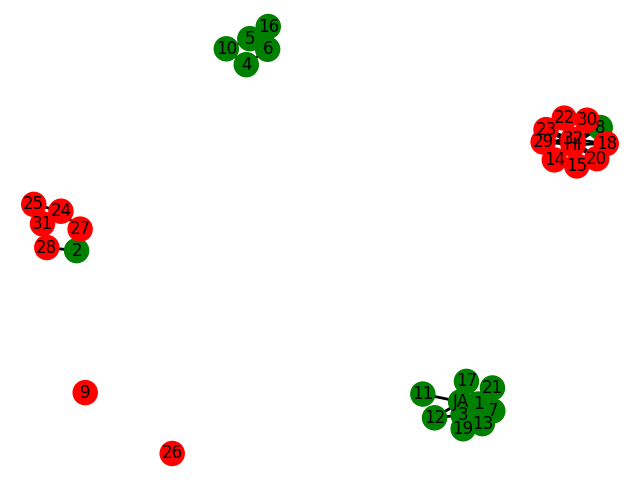
\includegraphics[scale=0.5]{resources/myplot21.png}
		\caption{ Split into 6 nodes }
	\end{figure}
	\begin{figure}[h!]
		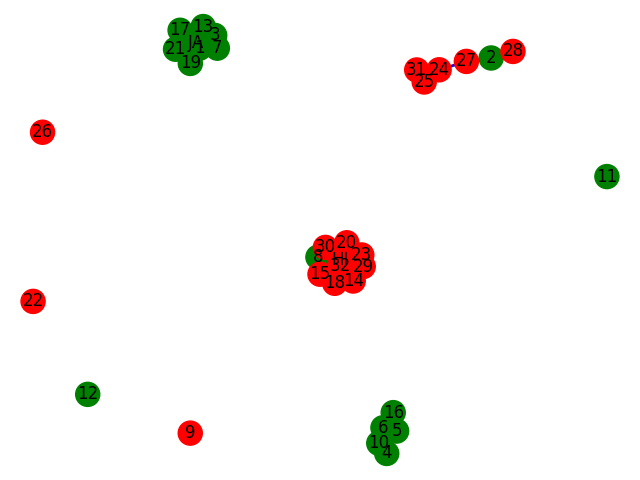
\includegraphics[scale=0.5]{resources/myplot22.png}
		\caption{Split into 10 groups }
	\end{figure}
	
	
\end{document}